
\begin{figure}
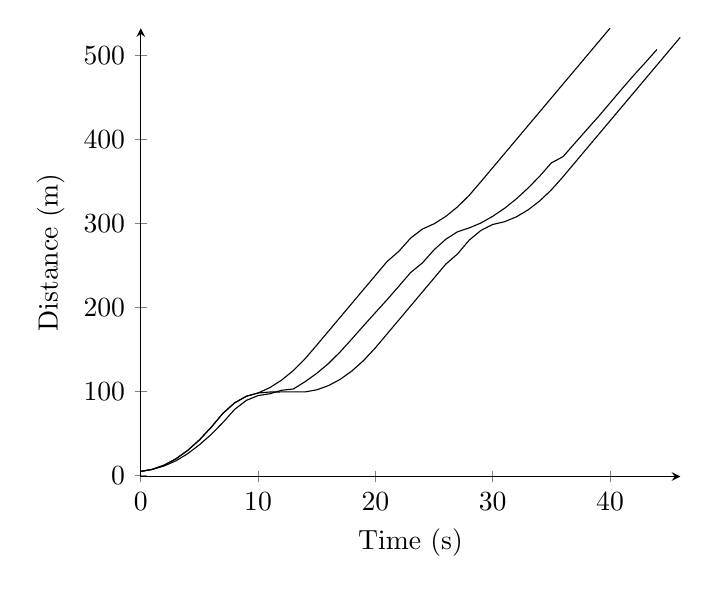
\begin{tikzpicture}
\begin{axis}[
legend style={
	anchor=west
},
axis x line=bottom,
axis y line=left,
ymin=-1,
point meta=explicit symbolic,
xlabel=Time (s),
ylabel=Distance (m)
]
\addplot[] coordinates {
(0, 5.1)
(1, 7.6)
(2, 12.6)
(3, 20.1)
(4, 30.1)
(5, 42.6)
(6, 57.6)
(7, 74.2)
(8, 86.6997297278)
(9, 94.5649106955)
(10, 98.4573862023)
(11, 99.6094044889)
(12, 99.7189990854)
(13, 99.7189990854)
(14, 99.7189990854)
(15, 102.218999085)
(16, 107.218999085)
(17, 114.718999085)
(18, 124.718999085)
(19, 137.218999085)
(20, 152.218999085)
(21, 168.818999085)
(22, 185.418999085)
(23, 202.018999085)
(24, 218.618999085)
(25, 235.218999085)
(26, 251.818999085)
(27, 263.958999085)
(28, 280.465265123)
(29, 292.028203901)
(30, 299.055158771)
(31, 302.295185543)
(32, 308.035212315)
(33, 316.275239087)
(34, 327.015265859)
(35, 340.25529263)
(36, 355.995319402)
(37, 372.595319402)
(38, 389.195319402)
(39, 405.795319402)
(40, 422.395319402)
(41, 438.995319402)
(42, 455.595319402)
(43, 472.195319402)
(44, 488.795319402)
(45, 505.395319402)
(46, 521.995319402)
};
\addplot[] coordinates {
(0, 5.1)
(1, 7.6)
(2, 12.6)
(3, 20.1)
(4, 30.1)
(5, 42.6)
(6, 57.6)
(7, 74.2)
(8, 86.6997297278)
(9, 94.5649106955)
(10, 98.4573862023)
(11, 104.849861709)
(12, 113.742337216)
(13, 125.134812723)
(14, 139.02728823)
(15, 155.419763737)
(16, 172.019763737)
(17, 188.619763737)
(18, 205.219763737)
(19, 221.819763737)
(20, 238.419763737)
(21, 255.019763737)
(22, 267.159763737)
(23, 282.795910232)
(24, 293.543718364)
(25, 299.852876728)
(26, 308.662035092)
(27, 319.971193456)
(28, 333.780351821)
(29, 350.089510185)
(30, 366.689510185)
(31, 383.289510185)
(32, 399.889510185)
(33, 416.489510185)
(34, 433.089510185)
(35, 449.689510185)
(36, 466.289510185)
(37, 482.889510185)
(38, 499.489510185)
(39, 516.089510185)
(40, 532.689510185)
};
\addplot[] coordinates {
(0, 5.1)
(1, 7.50275908931)
(2, 11.6205389488)
(3, 17.7435205067)
(4, 26.1927096548)
(5, 36.8205291404)
(6, 49.0223375483)
(7, 63.2548302656)
(8, 78.9031218017)
(9, 89.6607917909)
(10, 95.3890527628)
(11, 97.5488775892)
(12, 101.696620554)
(13, 103.194764767)
(14, 111.800530286)
(15, 121.827639675)
(16, 133.531056838)
(17, 147.435776809)
(18, 162.863114661)
(19, 178.668641664)
(20, 194.189623529)
(21, 209.583402093)
(22, 225.562566506)
(23, 241.828146615)
(24, 253.189778391)
(25, 268.896230792)
(26, 281.428381023)
(27, 290.381926516)
(28, 294.977226092)
(29, 300.862213217)
(30, 308.813817861)
(31, 318.168505689)
(32, 329.362403242)
(33, 342.184328144)
(34, 356.468965306)
(35, 372.382062596)
(36, 379.849436483)
(37, 395.80193258)
(38, 411.63059241)
(39, 427.275342919)
(40, 443.72033351)
(41, 460.219291246)
(42, 476.303184418)
(43, 491.657168701)
(44, 507.407933256)
};

\end{axis}
\end{tikzpicture}
\label{tik:50:14_V, 15_N, 17_S, 17_S.-60, 20_O, 21_O}
\caption{50 percent diving with GSC on route $14_V, 15_N, 17_S, 17_S.-60, 20_O, 21_O$}
\end{figure}
